\let\negmedspace\undefined
\let\negthickspace\undefined
\documentclass[journal]{IEEEtran}
\usepackage[a5paper, margin=10mm, onecolumn]{geometry}
%\usepackage{lmodern} % Ensure lmodern is loaded for pdflatex
\usepackage{tfrupee} % Include tfrupee package

\setlength{\headheight}{1cm} % Set the height of the header box
\setlength{\headsep}{0mm}  % Set the distance between the header box and the top of the text

\usepackage{gvv-book}
\usepackage{gvv}
\usepackage{circuitikz}
\usepackage{cite}
\usepackage{amsmath,amssymb,amsfonts,amsthm}
\usepackage{algorithmic}
\usepackage{graphicx}
\usepackage{textcomp}
\usepackage{xcolor}
\usepackage{txfonts}
\usepackage{listings}
\usepackage{enumitem}
\usepackage{mathtools}
\usepackage{gensymb}
\usepackage{comment}
\usepackage[breaklinks=true]{hyperref}
\usepackage{tkz-euclide} 
\usepackage{listings}
% \usepackage{gvv}                                        
\def\inputGnumericTable{}                                 
\usepackage[latin1]{inputenc}                                
\usepackage{color}                                            
\usepackage{array}                                            
\usepackage{longtable}                                       
\usepackage{calc}                                             
\usepackage{multirow}                                         
\usepackage{hhline}                                           
\usepackage{ifthen}                                           
\usepackage{lscape}
\usepackage{tikz}
\usetikzlibrary{patterns}
\begin{document}

\bibliographystyle{IEEEtran}
\vspace{3cm}


\title{GATE 2017 AE 40-52}
\author{ee24btech11015 - Dhawal}
\maketitle
% \maketitle
% \newpage
% \bigskip
{\let\newpage\relax\maketitle}

\renewcommand{\thefigure}{\theenumi}
\renewcommand{\thetable}{\theenumi}
\setlength{\intextsep}{10pt} % Space between text and floats




\begin{enumerate}[start=40]
\item A conventional low speed aircraft has the following aerodynamic characters:
\begin{align*}
    C_{D0}=0.020 \text{ and } e=10\brak{\text{Ostwald Constant}}
\end{align*}
The aircraft was flown to maintain a steady level flight and for minimum thrust required, at a lift coffecient of $C_L=0.8$. The numerical value of the aspect ratio of the wings is \rule{1cm}{0.4 pt} . (in three decimal places)

\item A batch of aluminum alloy yields in uniaxial tension at the stress of $330  \text{ MN/m}^2$. If this material is subjected to the following state of stress: $\sigma_x = 140  \text{ MN/m}^2, \sigma_y = -70  \text{ MN/m}^2, \sigma_z = 0,  \tau_{xy} = X \text{ MN/m}^2, \tau_{yz} = 0 \text{ and } \tau_{zx} = 0$. The value of $X$ that would result in yielding according to the Von Mises failure criterion is \rule{1cm}{0.4 pt} . (in three decimal places)

\item The roots obtained by solving longitudinal characteristic equations of motion for a statically stable aircraft are given below:
\begin{align*}
    \lambda_{1,2} = -0.02 \pm 0.30i, \; \lambda_{3,4} = -2.00 \pm 2.50i, \text{ where } i = \sqrt{-1} 
\end{align*} 
The undamped short-period longitudinal natural frequency (radians/sec) and damping ratio, in that order, are close to:
\begin{multicols}{4}
\begin{enumerate}
\item $3.40, 0.73$
\item  $3.36, 0.65$
\item  $3.83, 0.56$
\item  $3.20, 0.63$
\end{enumerate}
\end{multicols}

\item An aircraft is to be designed to ensure that it has enough excess power to achieve steady climb at flight path angle, $\gamma = 10$ degrees, maintaining $\frac{C_L}{C_D} = 1.0$. The numerical value of the thrust to weight ratio of the complete aircraft to meet the above requirement under standard atmospheric condition will be \rule{1cm}{0.4 pt} . (in three decimal places)

\item A conventional aircraft was analyzed to estimate the contribution of wing towards $C_{m0}\brak{C_m \text{ at } \alpha=0}$ of the whole aircraft. The wing had installed with zero setting angle along the fuselage reference line. Further, the wing was laid such that $\Bar{X}_{ac,w}=0.3 \text{ and } \Bar{X}_{cg,aircraft}=0.4. \: \Bar{X}_{ac,w} \text{ and } \Bar{X}_{cg,aircraft}$ are the non-dimensional distances, from the leading edge of the wing, of the aerodynamical center of the wing and center of gravity of the aircraft respectively. The wing had the following aerodynamic characteristics:
\begin{align*}
    C_{\text{L0}} = 0.20 \text{ and }  C_{\text{mac,wing}} = -0.02
\end{align*}

 The numerical value of the $C_{m0,w}$ (contribution of the wing to $C_{m0}$) about the CG of the aircraft is \rule{1cm}{0.4 pt} . (in two decimal places)

\item In a combustor, gaseous Octane $\brak{\text{C}_8\text{H}_{18}}$ and air are to be burned in stoichiometric proportions. If the required flow rate of air is $1$ kg/s, what should be the corresponding flow rate of Octane?
\begin{multicols}{4}
\begin{enumerate}
\item $0.066$ kg/s
\item  $15.15$ kg/s
\item  $0.16 $kg/s
\item  $6.25 $kg/s
\end{enumerate}
\end{multicols}



\item The given diagram represents the velocity triangles at the leading edge $\brak{1}$ and trailing edge $\brak{2}$ at the mean radius of a single stage axial compressor rotor. The stage efficiency of the compressor is $0.8$. The stagnation temperature of air entering the stage is $298 $K and the specific heat at constant pressure for air is $1.005 $kJ/kgK. The ratio of specific heats for air is $1.4$. Considering actual work in the rotor is equal to the ideal work, the pressure ratio for the stage is equal to \rule{1cm}{0.4 pt} . (in two decimal places)
\begin{center}
    
\begin{circuitikz}
\tikzstyle{every node}=[font=\LARGE]

\draw [dashed] (2.75,10.5) -- (2.75,3.5);
\draw [->, >=Stealth] (2.75,8.5) -- (9.5,9.75);
\draw [->, >=Stealth] (2.75,8.5) -- (9.5,8.75);
\draw [->, >=Stealth] (2.75,6) -- (9.25,9.5);
\draw [->, >=Stealth] (2.75,6) -- (9.5,6.25);
\draw [->, >=Stealth] (2.75,6) -- (9.5,3.75);
\draw [->, >=Stealth] (2.75,8.5) -- (9.25,4);
\draw [->, >=Stealth] (9.5,10.75) -- (9.5,3.5);
\node [font=\large] at (2.5,8.5) {2};
\node [font=\large] at (2.5,6) {};
\node [font=\large] at (2.5,6) {1};
\draw [->, >=Stealth] (4.5,3.25) -- (2.75,3.25);
\draw [->, >=Stealth] (8,3.25) -- (9.5,3.25);
\node [font=\Large] at (6.25,3.25) {$V_Z=165 m/s$};
\node [font=\Large] at (6.25,10.5) {$U=200 m/s$};
\node [font=\LARGE, rotate around={-172:(0,0)}] at (3.5,6.25) {$C$};
\node [font=\LARGE, rotate around={-178:(0,0)}] at (4.75,8.75) {$c$};
\node [font=\large] at (6.5,8.85) {$\beta_2=11\degree$};
\node [font=\LARGE] at (6,9) {};
\node [font=\LARGE] at (4.5,6.5) {};
\node [font=\large] at (4.75,6.5) {$\beta_1=45\degree$};
\end{circuitikz}
\end{center}


\item An aircraft with a turbojet engine, having an inlet area of $1{\text{m}}^2$, is flying at $270$ m/s at an altitude where the atmospheric pressure is equal to $0.9$ bar and the ambient temperature is equal to $290$ K. The stagnation pressure and temperature at the exit of the turbine are equal to $1.6 \text{bar} \text{ and } 774 $K respectively. The specific heat at constant pressure of the burned gases is equal to $1.147 $KJ/kgK and the ratio of specific heats is equal to $1.33$. Considering ideal expansion in the nozzle with no losses, the specific thrust produced by the engine is \rule{1cm}{0.4 pt} Ns/kg. (in one decimal place) 
 
\item Air, at $450$ K stagnation temperature and at a rate of $50 $kg/s, enters the combustor of a turbofan engine and is burned with $1$ kg/s of Aviation Kerosene (heating value $44$ MJ/kg). The specific heat of air at constant pressure for the incoming air and the burned products are $1.005 \text{kJ/kgK} \text{ and } 1.147 $kJ/kgK  respectively. Assuming $100\%$ burner efficiency, the stagnation temperature at the exit of the combustor is equal to \rule{1cm}{0.4 pt} K. (in one decimal place) 

\item A single stage chemical rocket, having an initial mass of $10,000 $kg and specific impulse of $450$ s, is launched from the surface of the earth and has to reach the escape velocity $11$ km/s at burn out. Consider $ g_e = 9.8 \, {\text{m/s}}^2 $. If the atmospheric drag and the effect of gravity are to be neglected, the mass of propellant to be carried by the rocket is equal to \rule{1cm}{0.4 pt} Kg. (in one decimal place) 

\item A centrifugal compressor requires $1800 $kW of power to compress $10 $kg/s of air. Consider the whirl velocity component is equal to the impeller speed (i.e., no slip) and no losses in the impeller. If the impeller has to rotate at $1900$ rad/s, the diameter of the impeller to be \rule{1cm}{0.4 pt} m. (in two decimal places) 

\item An aircraft wing is idealized as a cantilever beam of constant width and length $ l $ with a tip mass of weight $ W $ (Newtons) and has a uniformly distributed loading of $ q_0 $ (Newtons/m) as shown in the figure. Flexure rigidity  $= EI $ and $ q_0 l = 10 \, W $.
\begin{center}
    

\begin{tikzpicture}

    % Cantilever support (left end)
    \fill[gray] (-0.5, -0.2) rectangle (0, 0.7);
    \draw[thick] (0, -0.2) -- (0, 0.7);
    \node[anchor=east] at (-0.5, 0.25) {Cantilever support};

    % Beam
    \draw[thick] (0, 0.25) -- (6, 0.25); 
    \draw[thick] (0, 0.15) -- (6, 0.15);

    % Tip mass (circle at right end)
    \fill[black] (6, 0.2) circle (0.3);
    \node[anchor=west] at (6.4, 0.2) {Tip mass};

    % Distributed load arrows
    \foreach \x in {0.5, 1.5, 2.5, 3.5, 4.5, 5.5} {
        \draw[thick, ->] (\x, 0.25) -- (\x, 0.75);
    }
    
    % Load label
    \node[anchor=south] at (3, 0.75) {$q_0$};

    % Beam length annotation
    \draw[<->] (0, -0.3) -- (6, -0.3);
    \node at (3, -0.5) {$l$};

\end{tikzpicture}

\end{center}
The upward deflection of the tip of the aircraft wing under the given loading can be expressed as:
\begin{align*}
    \delta=k\frac{Wl^3}{EI}
\end{align*}
The value of $k$  is \rule{1cm}{0.4 pt} . (in three decimal places)


\item For the state of plane stress shown in the figure, the minimum principal stress is $ -7 \, {\text{MN/m}}^2 $. The normal stress $ \sigma_x  \text{ in } {\text{MN/m}}^2$ is equal to \rule{1cm}{0.4 pt} (round to nearest integer).

\begin{center}
\begin{circuitikz}
\tikzstyle{every node}=[font=\LARGE]
\node [font=\large] at (2.5,6) {};
\node [font=\LARGE] at (6,9) {};
\node [font=\LARGE] at (4.5,6.5) {};
\draw  (5.75,6.5) rectangle (8.75,3.75);
\draw [->, >=Stealth] (9.25,6.5) -- (9.25,3.75);
\draw [->, >=Stealth] (8.75,7) -- (5.75,7);
\draw [->, >=Stealth] (5.25,4) -- (5.25,6.5);
\draw [->, >=Stealth] (5.5,3.25) -- (9,3.25);
\draw [->, >=Stealth] (7.25,6.5) -- (7.25,8.25);
\draw [->, >=Stealth] (8.75,5) -- (10.5,5);
\draw [->, >=Stealth] (7.5,3.75) -- (7.5,2.5);
\draw [->, >=Stealth] (5.75,5) -- (4,5);
\node [font=\LARGE] at (8,8.5) {$21 MN/m^2$};
\node [font=\LARGE] at (11,5) {$\sigma_x$};
\node [font=\LARGE] at (10.5,3.5) {$56 MN/m^2$};
\end{circuitikz}

\end{center}



\end{enumerate}
\end{document}
